% \subfloat[Unstructured data]{%
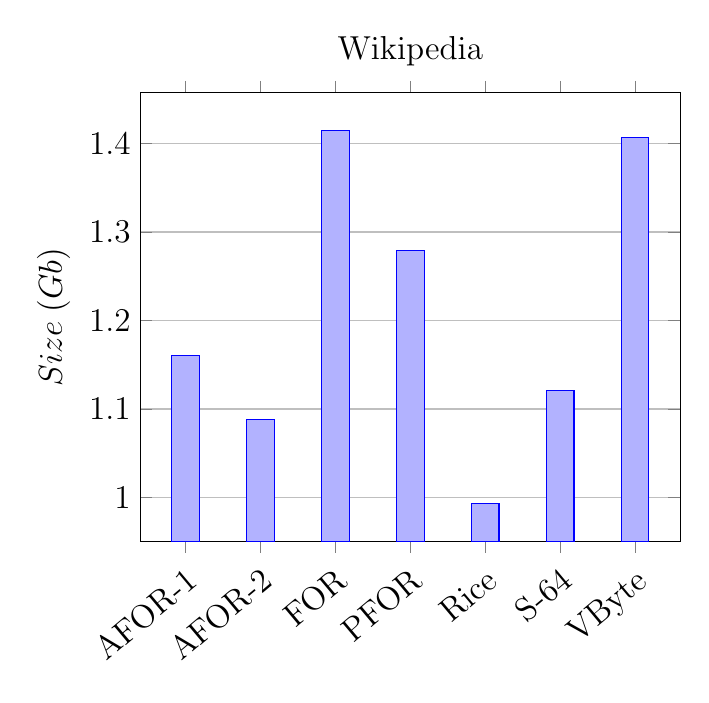
\begin{tikzpicture}[baseline]
\begin{axis}[
ylabel=$Size \; (Gb)$,
x tick label style={rotate=40, anchor=north east},
xtick={1,...,7},
xticklabels={AFOR-1, AFOR-2, FOR, PFOR, Rice, S-64, VByte},
legend style={at={(0.5,1.13)}, anchor=north, legend columns=-1},
label style={font=\large},
tick label style={font=\large},
title style={font=\large},
ybar,
ymajorgrids=true,
bar width=10pt,
title={Wikipedia},
%enlargelimits=0.15,
]
\addplot
coordinates {(1, 1.160) (2, 1.088) (3, 1.415) (4, 1.279) (5, 0.993) (6, 1.121)
(7, 1.407)};
\end{axis}
\end{tikzpicture}%

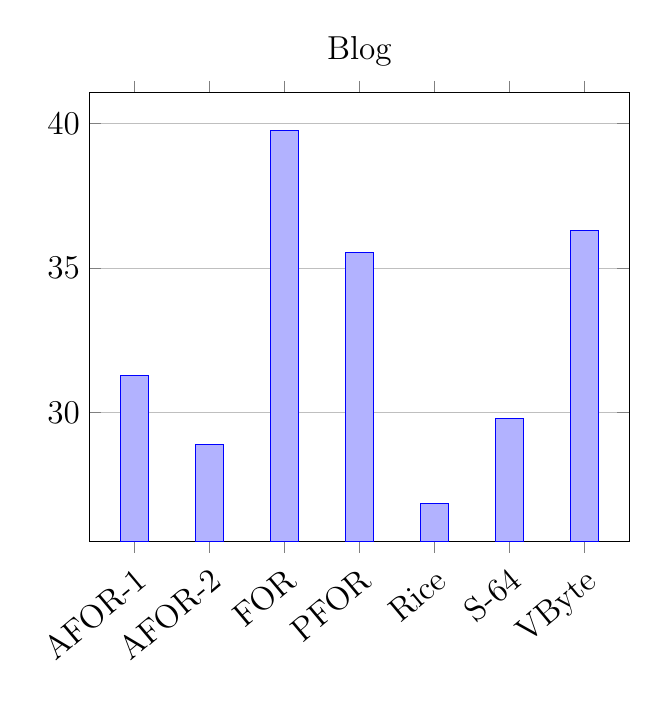
\begin{tikzpicture}[baseline]
\begin{axis}[
x tick label style={rotate=40, anchor=north east},
xtick={1,...,7},
xticklabels={AFOR-1, AFOR-2, FOR, PFOR, Rice, S-64, VByte},
legend style={at={(0.5,1.13)}, anchor=north, legend columns=-1},
label style={font=\large},
tick label style={font=\large},
title style={font=\large},
ybar,
ymajorgrids=true,
bar width=10pt,
title={Blog},
%enlargelimits=0.15,
]
\addplot
coordinates {(1, 31.292) (2, 28.895) (3, 39.777) (4, 35.536) (5, 26.851) (6,
29.800) (7, 36.303)};
\end{axis}
\end{tikzpicture}%
% }